% Options for packages loaded elsewhere
% Options for packages loaded elsewhere
\PassOptionsToPackage{unicode}{hyperref}
\PassOptionsToPackage{hyphens}{url}
\PassOptionsToPackage{dvipsnames,svgnames,x11names}{xcolor}
%
\documentclass[
  letterpaper,
  DIV=11,
  numbers=noendperiod,
  oneside]{scrartcl}
\usepackage{xcolor}
\usepackage[left=1in,marginparwidth=2.0666666666667in,textwidth=4.1333333333333in,marginparsep=0.3in]{geometry}
\usepackage{amsmath,amssymb}
\setcounter{secnumdepth}{-\maxdimen} % remove section numbering
\usepackage{iftex}
\ifPDFTeX
  \usepackage[T1]{fontenc}
  \usepackage[utf8]{inputenc}
  \usepackage{textcomp} % provide euro and other symbols
\else % if luatex or xetex
  \usepackage{unicode-math} % this also loads fontspec
  \defaultfontfeatures{Scale=MatchLowercase}
  \defaultfontfeatures[\rmfamily]{Ligatures=TeX,Scale=1}
\fi
\usepackage{lmodern}
\ifPDFTeX\else
  % xetex/luatex font selection
\fi
% Use upquote if available, for straight quotes in verbatim environments
\IfFileExists{upquote.sty}{\usepackage{upquote}}{}
\IfFileExists{microtype.sty}{% use microtype if available
  \usepackage[]{microtype}
  \UseMicrotypeSet[protrusion]{basicmath} % disable protrusion for tt fonts
}{}
\makeatletter
\@ifundefined{KOMAClassName}{% if non-KOMA class
  \IfFileExists{parskip.sty}{%
    \usepackage{parskip}
  }{% else
    \setlength{\parindent}{0pt}
    \setlength{\parskip}{6pt plus 2pt minus 1pt}}
}{% if KOMA class
  \KOMAoptions{parskip=half}}
\makeatother
% Make \paragraph and \subparagraph free-standing
\makeatletter
\ifx\paragraph\undefined\else
  \let\oldparagraph\paragraph
  \renewcommand{\paragraph}{
    \@ifstar
      \xxxParagraphStar
      \xxxParagraphNoStar
  }
  \newcommand{\xxxParagraphStar}[1]{\oldparagraph*{#1}\mbox{}}
  \newcommand{\xxxParagraphNoStar}[1]{\oldparagraph{#1}\mbox{}}
\fi
\ifx\subparagraph\undefined\else
  \let\oldsubparagraph\subparagraph
  \renewcommand{\subparagraph}{
    \@ifstar
      \xxxSubParagraphStar
      \xxxSubParagraphNoStar
  }
  \newcommand{\xxxSubParagraphStar}[1]{\oldsubparagraph*{#1}\mbox{}}
  \newcommand{\xxxSubParagraphNoStar}[1]{\oldsubparagraph{#1}\mbox{}}
\fi
\makeatother


\usepackage{longtable,booktabs,array}
\usepackage{calc} % for calculating minipage widths
% Correct order of tables after \paragraph or \subparagraph
\usepackage{etoolbox}
\makeatletter
\patchcmd\longtable{\par}{\if@noskipsec\mbox{}\fi\par}{}{}
\makeatother
% Allow footnotes in longtable head/foot
\IfFileExists{footnotehyper.sty}{\usepackage{footnotehyper}}{\usepackage{footnote}}
\makesavenoteenv{longtable}
\usepackage{graphicx}
\makeatletter
\newsavebox\pandoc@box
\newcommand*\pandocbounded[1]{% scales image to fit in text height/width
  \sbox\pandoc@box{#1}%
  \Gscale@div\@tempa{\textheight}{\dimexpr\ht\pandoc@box+\dp\pandoc@box\relax}%
  \Gscale@div\@tempb{\linewidth}{\wd\pandoc@box}%
  \ifdim\@tempb\p@<\@tempa\p@\let\@tempa\@tempb\fi% select the smaller of both
  \ifdim\@tempa\p@<\p@\scalebox{\@tempa}{\usebox\pandoc@box}%
  \else\usebox{\pandoc@box}%
  \fi%
}
% Set default figure placement to htbp
\def\fps@figure{htbp}
\makeatother





\setlength{\emergencystretch}{3em} % prevent overfull lines

\providecommand{\tightlist}{%
  \setlength{\itemsep}{0pt}\setlength{\parskip}{0pt}}



 


% load packages
\usepackage{geometry}
\usepackage{xcolor}
\usepackage{eso-pic}
\usepackage{fancyhdr}
\usepackage{sectsty}
\usepackage{fontspec}
\usepackage{titlesec}

%% Set page size with a wider right margin
\geometry{a4paper, total={170mm,257mm}, left=20mm, top=20mm, bottom=20mm, right=50mm}

%% Let's define some colours
\definecolor{light}{HTML}{E6E6FA}
\definecolor{highlight}{HTML}{800080}
\definecolor{dark}{HTML}{330033}

%% Let's add the border on the right hand side 
% \AddToShipoutPicture{% 
%     \AtPageLowerLeft{% 
%         \put(\LenToUnit{\dimexpr\paperwidth-3cm},0){% 
%             \color{light}\rule{3cm}{\LenToUnit\paperheight}%
%           }%
%      }%
%      % logo
%     \AtPageLowerLeft{% start the bar at the bottom right of the page
%         \put(\LenToUnit{\dimexpr\paperwidth-2.25cm},27.2cm){% move it to the top right
%             \color{light}
\includegraphics[width=1.5cm]{_extensions/nrennie/PrettyPDF/logo.png}
%           }%
%      }%
% }

%% Style the page number
\fancypagestyle{mystyle}{
  \fancyhf{}
  \renewcommand\headrulewidth{0pt}
  \fancyfoot[R]{\thepage}
  \fancyfootoffset{3.5cm}
}
\setlength{\footskip}{20pt}

%% style the chapter/section fonts
\chapterfont{\color{dark}\fontsize{20}{16.8}\selectfont}
\sectionfont{\color{dark}\fontsize{20}{16.8}\selectfont}
\subsectionfont{\color{dark}\fontsize{14}{16.8}\selectfont}
\titleformat{\subsection}
  {\sffamily\Large\bfseries}{\thesection}{1em}{}[{\titlerule[0.8pt]}]
  
% left align title
\makeatletter
\renewcommand{\maketitle}{\bgroup\setlength{\parindent}{0pt}
\begin{flushleft}
  {\sffamily\huge\textbf{\MakeUppercase{\@title}}} \vspace{0.3cm} \newline
  {\Large {\@subtitle}} \newline
  \@author
\end{flushleft}\egroup
}
\makeatother

%% Use some custom fonts
\setsansfont{Ubuntu}[
    Path=_extensions/nrennie/PrettyPDF/Ubuntu/,
    Scale=0.9,
    Extension = .ttf,
    UprightFont=*-Regular,
    BoldFont=*-Bold,
    ItalicFont=*-Italic,
    ]

\setmainfont{Ubuntu}[
    Path=_extensions/nrennie/PrettyPDF/Ubuntu/,
    Scale=0.9,
    Extension = .ttf,
    UprightFont=*-Regular,
    BoldFont=*-Bold,
    ItalicFont=*-Italic,
    ]
\KOMAoption{captions}{tableheading}
\makeatletter
\@ifpackageloaded{caption}{}{\usepackage{caption}}
\AtBeginDocument{%
\ifdefined\contentsname
  \renewcommand*\contentsname{Table of contents}
\else
  \newcommand\contentsname{Table of contents}
\fi
\ifdefined\listfigurename
  \renewcommand*\listfigurename{List of Figures}
\else
  \newcommand\listfigurename{List of Figures}
\fi
\ifdefined\listtablename
  \renewcommand*\listtablename{List of Tables}
\else
  \newcommand\listtablename{List of Tables}
\fi
\ifdefined\figurename
  \renewcommand*\figurename{Figure}
\else
  \newcommand\figurename{Figure}
\fi
\ifdefined\tablename
  \renewcommand*\tablename{Table}
\else
  \newcommand\tablename{Table}
\fi
}
\@ifpackageloaded{float}{}{\usepackage{float}}
\floatstyle{ruled}
\@ifundefined{c@chapter}{\newfloat{codelisting}{h}{lop}}{\newfloat{codelisting}{h}{lop}[chapter]}
\floatname{codelisting}{Listing}
\newcommand*\listoflistings{\listof{codelisting}{List of Listings}}
\makeatother
\makeatletter
\makeatother
\makeatletter
\@ifpackageloaded{caption}{}{\usepackage{caption}}
\@ifpackageloaded{subcaption}{}{\usepackage{subcaption}}
\makeatother
\makeatletter
\@ifpackageloaded{tcolorbox}{}{\usepackage[skins,breakable]{tcolorbox}}
\makeatother
\makeatletter
\@ifundefined{shadecolor}{\definecolor{shadecolor}{rgb}{.97, .97, .97}}{}
\makeatother
\makeatletter
\@ifundefined{codebgcolor}{\definecolor{codebgcolor}{named}{light}}{}
\makeatother
\makeatletter
\ifdefined\Shaded\renewenvironment{Shaded}{\begin{tcolorbox}[sharp corners, boxrule=0pt, colback={codebgcolor}, enhanced, frame hidden, breakable]}{\end{tcolorbox}}\fi
\makeatother
\makeatletter
\@ifpackageloaded{sidenotes}{}{\usepackage{sidenotes}}
\@ifpackageloaded{marginnote}{}{\usepackage{marginnote}}
\makeatother
\usepackage{bookmark}
\IfFileExists{xurl.sty}{\usepackage{xurl}}{} % add URL line breaks if available
\urlstyle{same}
\hypersetup{
  colorlinks=true,
  linkcolor={highlight},
  filecolor={Maroon},
  citecolor={Blue},
  urlcolor={highlight},
  pdfcreator={LaTeX via pandoc}}


\author{}
\date{}
\begin{document}

\pagestyle{mystyle}


\section{W2: Simulation \& Pastiche:
Postmodernism}\label{w2-simulation-pastiche-postmodernism}

\href{https://store.nonesuch.com/products/visions-and-miracles-digital-mp3-album}{\pandocbounded{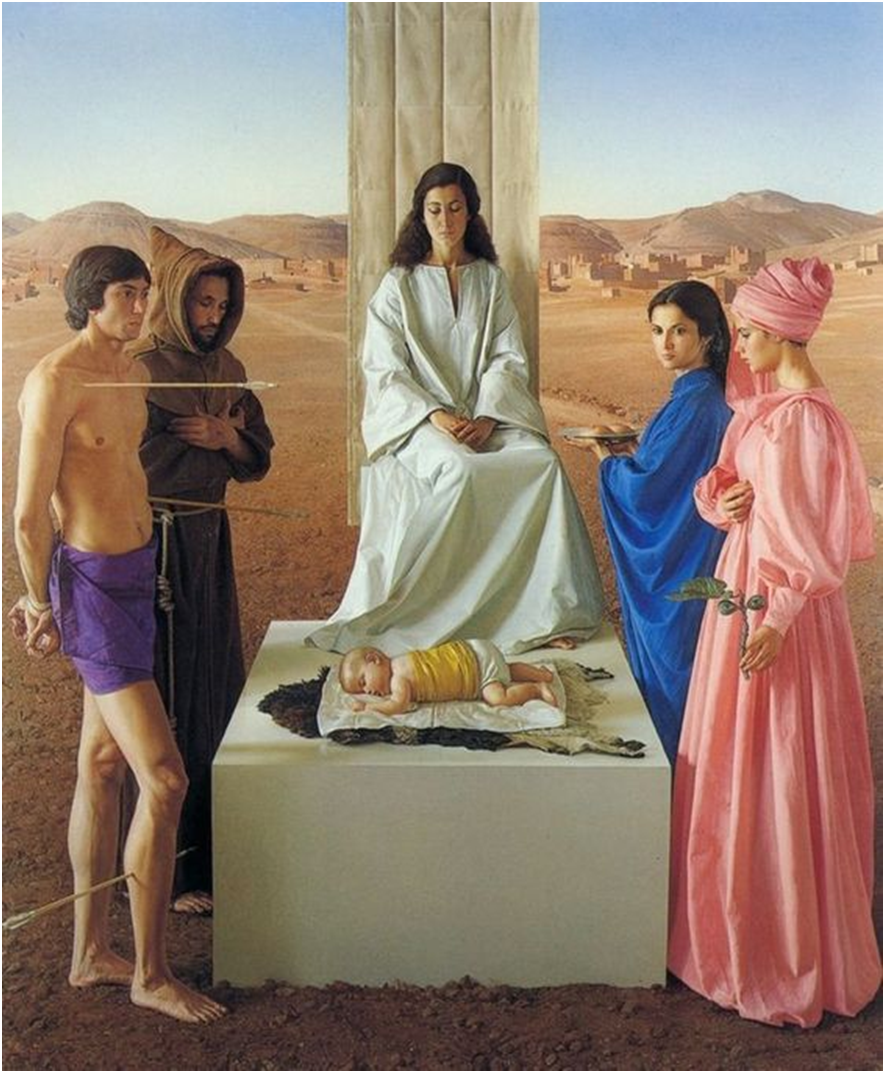
\includegraphics[keepaspectratio]{img/claudio-bravo-madonna.png}}}

\marginnote{\begin{footnotesize}

\href{http://amaliaulman.eu/}{Amalia
Ulman};~\href{https://www.instagram.com/amaliaulman/}{Instagram}
Alastair Sooke,
``\href{http://www.telegraph.co.uk/photography/what-to-see/is-this-the-first-instagram-masterpiece/}{Is
This The First Instagram Masterpiece?}'' (\textbf{The Telegraph}, 18
January 2016)
``\href{http://www.dazeddigital.com/artsandculture/article/23700/1/amalia-ulman-meme-come-true}{Amalia
Ulman: Meme Come True}'' (\textbf{Dazed}) Emilie Friedlander,
``\href{http://www.thefader.com/2014/11/07/social-anxiety-why-amalia-ulmans-middlebrow-instagram-feed-is-no-different-from-yours}{Social
Anxiety: Why Amalia Ulman's Fake `Middlebrow' Instagram Is No Different
From Yours},'' (\textbf{Fader}, 7 November 2014)

To watch:

\href{https://www.justwatch.com/us/movie/el-planeta}{\textbf{El
Planeta}}~(Amalia Ulman, 2020)
\href{https://www.netflix.com/search?q=inventing\%20anna&jbv=81008305}{\textbf{Inventing
Anna}}, episode 6 (Netflix, 2022)

\end{footnotesize}}

\href{https://en.wikipedia.org/wiki/Claudio_Bravo_(painter)}{Claudio
Bravo}, \textbf{Madonna} (1979)

You've heard of postmodernism, of course---who hasn't? As arguably the
most influential cultural movement of the past half century, it's almost
inescapable today, ubiquitous across the spectrum of the arts, from
Warhol to Jeff Koons, \textbf{Twin Peaks} to \textbf{Stranger Things},
Quentin Tarantino's \textbf{Pulp Fiction} to Wes Anderson's \textbf{Isle
of Dogs}---okay that's enough, I could go on for the entire
lecture\ldots{}

But what exactly \textbf{is} postmodernism? When did it start? And has
it ended yet? In keeping with my approach in the course thus far, rather
than plunging into dense theoretical texts, we will explore
postmodernist aesthetics through some representative examples---in this
case the works of the U.S. artist
\href{https://www.artnet.com/artists/cindy-sherman/}{Cindy Sherman} and
the more recent Argentinian artist \href{http://amaliaulman.eu/}{Amalia
Ulman}.

Since there simply isn't sufficient space here to explore all of the
many facets of postmodernism, some basic distinctions and pointers will
have to suffice. For a deeper dive, your starting point should probably
be Fredric Jameson's influential essay, ``Postmodernism or the Cultural
Logic of Late Capitalism'', followed by his book; or the French social
theorist Jean Baudrillard's classic book \textbf{Simulacra and
Simulations}. But you don't have to start with either of these texts.
The first book I read on postmodernism was actually about architecture,
Charles Jenks's book \textbf{The Language of Postmodernist
Architecture}, which has some illuminating discussion of the differences
between modernist and postmodernist architecture.

An initial distinction is useful between postmodern\textbf{ism}, which
refers to an aesthetic movement extending across the spectrum of the
arts, and postmodern\textbf{ity}, a broader term that refers to a
general \textbf{condition} (the reference points here being
Jean-François Lyotard's influential book The \textbf{Postmodern
Condition} and David Harvey's \textbf{The Condition of Postmodernity})
of society that has come to characterize the experience of global
societies in the second half of the twentieth century and the first part
of the twenty-first. I'm not going to get into the nature of
postmodernity here, but suffice to say that postmodernism in the arts
can be thought of as the artistic and cultural counterpart of the
conditon of postmodernity itself.

What follows can be considered a kind of ``Postmodernism 101'' that
assumes that you know very little about postmodernism at the outset, and
suggests some lines of inquiry to follow if you're interested in
exploring it in more depth.

So what do the diverse group of artists mentioned so far---Andy Warhol,
Cindy Sherman, David Lynch, Quentin Tarantino, Jeff Koons, Wes Anderson,
Amalia Ulman, and many more---have in common, aesthetically speaking?

While people who have tried to define postmodernism agree that it can
mean many different things, most would agree that one of its defining
characteristics is \textbf{pastiche}, or what Fredric Jameson called
``blank parody''. Pastiche here refers to \textbf{the mimicry of
particular historical styles}, irrespective of the artistic field in
question---painting, architecture, cinema, television, music, comics,
and so on.

Consider, for example, the image at the top of this page,
\textbf{Madonna} by the Chilean artist
\href{https://en.wikipedia.org/wiki/Claudio_Bravo_(painter)}{Claudio
Bravo}. At first glance, you might easily mistake it for a Renaissance
painting, in terms of its apparently religious subject matter, the
vaguely biblical background that recalls religious illustrated books,
and the symmetrical composition. The figure on the left pierced with
arrows, for example, recalls the Christian martyr St.~Sebastian, the
subject of numerous Renaissance paintings. It might come as a surprise,
then, to learn that the painting is a contemporary one (1979). The image
first came to my attention in the early 1990s when it was used on the
cover of an album by the
\href{https://www.kitka.org/ensemble-alcatraz}{Ensemble Alcatraz},
\textbf{Visions and Miracles} (1988), a vocal group specializing in
medieval and early modern music based in the San Franciso Bay area. The
label website describes the album thus:

\begin{quote}
\emph{The Iberian Peninsula in the 13th century was home to a great
exchange of cultures. One result: the }cantiga\emph{, a combination of
old and new musics from Christian, Muslim, and Jewish sources that told
stories of adventure, calamity, and redemption, here brought to life by
the Ensemble Alcatraz.}
\end{quote}

In Claudio Bravo's pastiche of Renaissance painting, and the Ensemble
Alcatraz's eclectic pastiches of 13th-century Iberian music, we are
already deeply immersed in postmodernist aesthetics.
{\marginnote{\begin{footnotesize}One of the characteristics of
postmodernist painting is a return to figurative representation, in
reaction against the abstraction that was one of the hallmarks of
modernist painting, from the geometric minimalism of Mondrian to the
abstract expressionism of Jackson Pollock.\end{footnotesize}}}

One could spend a lot of time exploring postmodernist aesthetics simply
within painting, from the 1960s ``Pop Art'' of Andy Warhol and Roy
Lichtenstein to more recent examples. Both of these artists exemplify
another key principle of postmodernist aesthetics: the embrace of
popular media such as comics and the mass-cultural imagery of
advertising, collapsing the modernist hierarchy between ``high''
(avant-garde) art and the ``low'' art (kitsch) of consumer mass culture.

Rather than painting, a particularly interesting starting point for
exploring postmodernist aesthetics is photography. The 1970s saw the
emergence of a number of female artists whose work engaged in different
ways with photography as a means of elaborating a new, postmodernist
aesthetics. They included Jenny Holzer, Barbara Kruger, Sherrie Levine,
or Sandy Skoglund (I leave you to Google any of these), but the two
artists that I'm going to discuss today are of particular interest
because of how their photographic work engages with the cinematic (Cindy
Sherman) and social media (Amalia Ulman).

\subsubsection{\texorpdfstring{\href{https://www.artnet.com/artists/cindy-sherman/}{Cindy
Sherman}}{Cindy Sherman}}\label{cindy-sherman}

Cindy Sherman is best known for her series of photographs (I think there
are over 70 in all) dating from the late 1970s (1977-80) in which she
elaborately stages stereotypical female roles that look uncannily like
they are film stills from popular movies---the only difference being
that the movies in question don't exist. The main image for the course
syllabus is a collage of some of the best-known of these photographs.
Take a closer look at it, and click on the image to find out more about
the series.

\href{https://www.moma.org/interactives/exhibitions/1997/sherman/index.html}{\pandocbounded{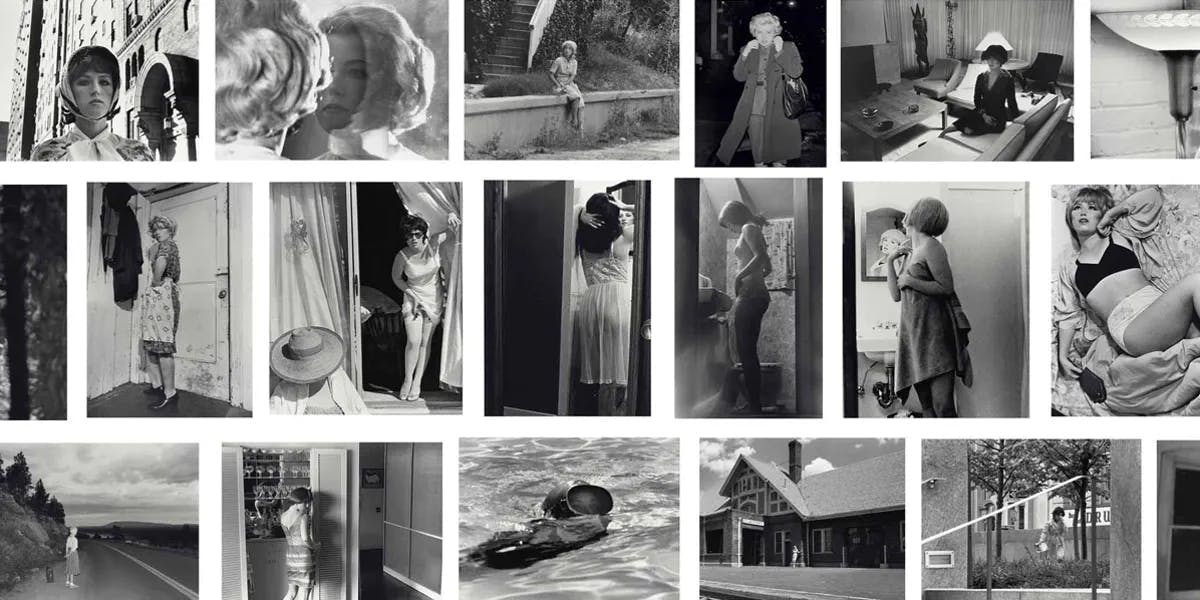
\includegraphics[keepaspectratio]{img/cindy-sherman.jpg}}}

So what is ``postmodernist'' about this project? First, and related to
the earlier discussion, because as the title of the series itself
(\textbf{Untitled Film Stills}) makes clear, the photographs pastiche
(that is, mimic or imitate) the visual style of the film still as a
media \textbf{format} often seen in newspapers, magazines, and
promotional matierals (such as film posters). In addition to the
photographs' formal mimicry of the film still, moreover, they also
pastiche the visual style of popular films genres often problematized
for their stereotypical portrayals of women, notably the well-known
\emph{femme fatale} stereotype of 1940s-1950s \emph{film noir}. Some of
Cindy Sherman's photographs can be seen as pastiching the \textbf{visual
codes} of \emph{film noir}, most obviously in her decision to shoot on
black-and-white film stock, reproducing the monochromatic look that is
one of the most striking visual characteristics of \emph{film noir}. It
should be remembered that while the default film stock for photographers
(especially photojournalists) well into the 1960s was black and white,
even though shooting in color had been technically possible long before
then, by the 1970s color had so become the norm that to choose to shoot
in black and white already lent a \textbf{retro} that has become one of
the hallmarks of postmodernist aesthetics. Sherman's decision to shoot
in black and white, then, is another (easily overlooked) element of
their stylistic pastiche of the monochromatic aesthetic both of
\emph{film noir} and historical photography.

What's so fascinating about Sherman's film stills, though, is that even
though some of them can be seen as stylistic pastiches of \emph{film
noir}, in many other photographs it's far less clear which cinematic
genre is the object of pastiche. While there's often a strong visual
sense of \emph{déjà vu}, evoking a popular film of the 1950s or 1960s,
they key point is the \textbf{indeterminacy} of the reference---the fact
that we can't identify the photograph with any specific historical film
or film genre.

This brings us to another defining concept of postmodernist aesthetics:
\textbf{simulation}. The concept was elaborated in several classic
essays in the 1970s by the French social theorist Jean Baudrillard,
notably in his book (mentioned earler) \textbf{Simulacra and
Simulations} (1979). For Baudrillard, the postmodern world is dominated
by what he calls \textbf{simulacra} (sing. ``simulacrum''), a new form
of representation that essentially reverses the hierarchical
relationship between the model and the copy. Historically, in the
history of art, the model---in the form of the original work of
art---has always preceded the copy: there is only one Mona Lisa, even
though there are thousands of copies of Leonardo Da Vinci's
painting.{\marginnote{\begin{footnotesize}This is why the Mona Lisa has
what Walter Benjamins calls \textbf{aura}, its historical uniqueness in
space and time\end{footnotesize}}}. The age of what Baudrillard calls
the simulacrum---the postmodernist age---is defined by the reversal of
this hierarchy, by the ascendancy of \textbf{copies without models}
(which is what Baudrillard means by simulacra). Whereas in the era of
realism, what was still understood as the ``real world'' preceded
representation of it (regardless of the medium---literature, painting,
photography, cinema, TV), by the 1970s, Baudrillard argued, the
relationship between the real and representation had reversed, or
perhaps more accurately the distinction between the two had collapsed:
henceforth, claimed Baudrillard, ``reality'' had become effectively
indistinguishable from mass-media representations of it, or what he and
the Italian semiotic theorist Umberto Eco called \textbf{hyperreality}.

We don't need to go any further at this point to understand how the
photography of Cindy Sherman, as well as many other artists like her in
the 1970s, could be seen as an artistic commentary on the hyperrealist
world that Baudrillard was describing. Sherman's Film Stills photographs
are also copies without models in the sense that what semiotic theorists
would call their \textbf{referent}---the original film from which they
are sourced---does not exist. They are what Baudrillard might call
cinematic simulacra.

Over the past few decades, Cindy Sherman has become increasingly revered
as one of the most influential figures in the emergence of postmodernist
aesthetics since the 1970s. Her photographic critique of stereotypical
representations of women in popular cinema was part of the larger
current of feminist critiques of patriarchal representation, from Laura
Mulvey's influential critique of the male gaze in her mid-1970s essay to
Chantal Akerman's groundbreaking film \textbf{Jeanne Dielman, 23 quai du
Commerce, 1080 Bruxelles} (1975). Sherman has continued her exploration
of female representation right up to the present, and even has an
Instagram account. An episode of the recent Netflix series
\textbf{Inventing Anna} includes an episode in which characters discuss
her work at a gallery retrospective, and includes a brief cameo by
Sherman herself, wearing the same head-scarfed outfit that she wears in
one of her original Film Stills photographs, essentially re-enacting her
own earlier roleplay in the photograph. (Could it be any more
postmodernist?!?). The inclusion of Sherman in the show could scarcely
be more appropriate, given that its subject is Anna Sorokin, who conned
luxury hotels and her wealthy New York socialite friends by masquerading
as a German heiress called Anna Delvey--another stunningly postmodernist
example of ``representation'' usurping the place of reality.

\subsubsection{\texorpdfstring{\href{http://amaliaulman.eu/}{Amalia
Ulman}}{Amalia Ulman}}\label{amalia-ulman}

Cindy Sherman's
\href{https://www.instagram.com/cindyshermancomplete/}{Instagram}
account (in fact, she has several) provides a link between her 1970s
performance-art photography exploring female identity and the work of
the social media artist Amalia Ulman, which can arguably be seen as
continuing Sherman's project in the twenty-first century domain of
social media. If you read any of the articles about Ulman's work linked
to as this week's reading assignments, you should by now have a good
idea of how she fits into the larger framework of postmodernism that I
have been sketching out in the preceding discussion. As with Sherman's
Film Stills, and as with a number of similar postmodernist feminist
artists (the French artist
\href{https://www.newyorker.com/books/under-review/sophie-calle-and-the-art-of-leaving-a-trace}{Sophie
Calle} is another example), in her fake Instagram account Ulman
fabricated a stereotypical female persona as an art project, exposing
through the sexist comments of her male admirers the continuing pressure
on young women to conform to the visual pleasure of the male gaze almost
half a century since Laura Mulvey's critique, and in spite of
``postfeminist'' celebrations of the power of female sexuality Ulman's
work can in fact be seen as developing such as critique through
masquerade, photography, and social media platforms in a manner that
continues the artistic critiques of so many other postmodernist feminist
artists since the 1970s.

Just as Cindy Sherman's Film Stills project explored stereotypical
representations of women in cinema, Amalia Ulman has recently gone a
step further by directing her first feature film, \textbf{El Planeta},
that continues her exploration of representations of female identity in
the social media age more directly in cinematic form. The film's opening
sequence again sees Ulman role-playing, this time posing as a call girl
negotiating sexual and financial arrangements with a future client in
what subsequently proves to be (like her Instagram persona) a pure
fabrication that ruthlessly exposes the objectification of women in
patriarchal society. The masquerades continue after this initial one,
from her later (apparent) impersonation of an international designer to
her later romantic roleplay in her date with the Asian guy that she
meets in the gift shop. Both she herself and her mother (played, in
fact, by Ulman's own mother), it turns out, are engaged in role-playing
a fantasy of a glamorious lifestyle that has no relation to their
impoverished socio-economic reality---a masquerade that is ultimately
exposed in the mother's arrest for shoplifting with which the film ends.

It's worth noting, finally, that as with Cindy Sherman's film stills,
Ulman's 2022 film is also in black and white, stylistically pastiching
not \emph{film noir} in this case but the French New Wave films of
Jean-Luc Godard, Agnès Varda, or François Truffaut, many of which also
engage with the problematic position of women in the French society of
their time. It's interesting in this regard to think about the
relationship between \textbf{El Planeta} and Varda's film \textbf{Cléo
from 5 to 7}, or Godard's film with Anna Karina, \textbf{Vivre Sa Vie}
which explores themes similar to those in Ulman's film. I leave you to
think about those connections, but suffice to say that Ulman's
black-and-white pastiche of a New Wave film also attests to the legacy
of postmodernist aesthetics half a century after Cindy Sherman's iconic
film stills.




\end{document}
